\documentclass[border=2mm]{standalone}
\usepackage{tikz}
\usetikzlibrary{calc}

\begin{document}


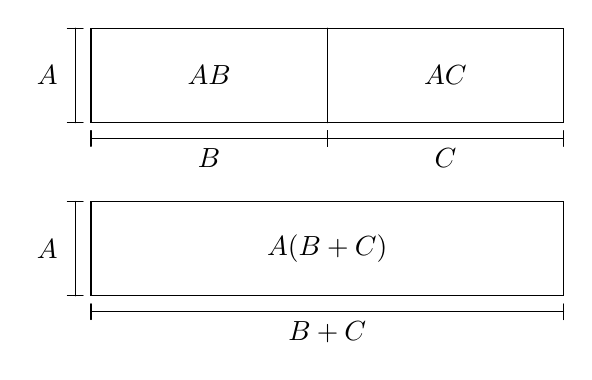
\begin{tikzpicture}[x=1cm,y=1cm,line cap=round]

%======================= HÌNH TRÊN =======================%

% khung AB | AC
\draw (1,4) rectangle (7,5.2);
\draw (4,4) -- (4,5.2);

% nhãn trong hình
\node at (2.5,4.6) {$AB$};
\node at (5.5,4.6) {$AC$};

% ngoặc đứng A
\draw (0.8,4) -- (0.8,5.2);
\draw (.7,5.2) -- (.9,5.2);
\draw (.7,4) -- (.9,4);
\node[left] at (0.7,4.6) {$A$};

% đoạn đo B (vạch nhỏ gọn)
\draw (1,3.8) -- (4,3.8);
\draw (1,3.8) ++(0,0.10) -- ++(0,-0.20);
\draw (4,3.8) ++(0,0.10) -- ++(0,-0.20);
\node[below] at (2.5,3.8) {$B$};

% đoạn đo C
\draw (4,3.8) -- (7,3.8);
\draw (4,3.8) ++(0,0.10) -- ++(0,-0.20);
\draw (7,3.8) ++(0,0.10) -- ++(0,-0.20);
\node[below] at (5.5,3.8) {$C$};

%======================= HÌNH DƯỚI =======================%

% khung A(B+C) – dịch xuống để cách hình trên
\draw (1,1.8) rectangle (7,3.0);
\node at (4,2.4) {$A(B + C)$};

% ngoặc đứng A
\draw (0.8,1.8) -- (0.8,3);
\draw (.7,3) -- (.9,3);
\draw (.7,1.8) -- (.9,1.8);
\node[left] at (0.7,2.4) {$A$};

% đoạn đo B+C
\draw (1,1.6) -- (7,1.6);
\draw (1,1.6) ++(0,0.10) -- ++(0,-0.20);
\draw (7,1.6) ++(0,0.10) -- ++(0,-0.20);
\node[below] at (4,1.6) {$B + C$};

\end{tikzpicture}


\end{document}